% This is "sig-alternate.tex" V2.1 April 2013
% This file should be compiled with V2.5 of "sig-alternate.cls" May 2012
%
% This example file demonstrates the use of the 'sig-alternate.cls'
% V2.5 LaTeX2e document class file. It is for those submitting
% articles to ACM Conference Proceedings WHO DO NOT WISH TO
% STRICTLY ADHERE TO THE SIGS (PUBS-BOARD-ENDORSED) STYLE.
% The 'sig-alternate.cls' file will produce a similar-looking,
% albeit, 'tighter' paper resulting in, invariably, fewer pages.
%
% ----------------------------------------------------------------------------------------------------------------
% This .tex file (and associated .cls V2.5) produces:
%       1) The Permission Statement
%       2) The Conference (location) Info information
%       3) The Copyright Line with ACM data
%       4) NO page numbers
%
% as against the acm_proc_article-sp.cls file which
% DOES NOT produce 1) thru' 3) above.
%
% Using 'sig-alternate.cls' you have control, however, from within
% the source .tex file, over both the CopyrightYear
% (defaulted to 200X) and the ACM Copyright Data
% (defaulted to X-XXXXX-XX-X/XX/XX).
% e.g.
% \CopyrightYear{2007} will cause 2007 to appear in the copyright line.
% \crdata{0-12345-67-8/90/12} will cause 0-12345-67-8/90/12 to appear in the copyright line.
%
% ---------------------------------------------------------------------------------------------------------------
% This .tex source is an example which *does* use
% the .bib file (from which the .bbl file % is produced).
% REMEMBER HOWEVER: After having produced the .bbl file,
% and prior to final submission, you *NEED* to 'insert'
% your .bbl file into your source .tex file so as to provide
% ONE 'self-contained' source file.
%
% ================= IF YOU HAVE QUESTIONS =======================
% Questions regarding the SIGS styles, SIGS policies and
% procedures, Conferences etc. should be sent to
% Adrienne Griscti (griscti@acm.org)
%
% Technical questions _only_ to
% Gerald Murray (murray@hq.acm.org)
% ===============================================================
%
% For tracking purposes - this is V2.0 - May 2012

\documentclass{sig-alternate-05-2015}

\begin{document}

% Copyright
\setcopyright{acmcopyright}
%\setcopyright{acmlicensed}
%\setcopyright{rightsretained}
%\setcopyright{usgov}
%\setcopyright{usgovmixed}
%\setcopyright{cagov}
%\setcopyright{cagovmixed}


% DOI
\doi{10.475/123_4}

% ISBN
\isbn{123-4567-24-567/08/06}

%Conference
\conferenceinfo{PLDI '13}{June 16--19, 2013, Seattle, WA, USA}

\acmPrice{\$15.00}

%
% --- Author Metadata here ---
\conferenceinfo{WOODSTOCK}{'97 El Paso, Texas USA}
%\CopyrightYear{2007} % Allows default copyright year (20XX) to be over-ridden - IF NEED BE.
%\crdata{0-12345-67-8/90/01}  % Allows default copyright data (0-89791-88-6/97/05) to be over-ridden - IF NEED BE.
% --- End of Author Metadata ---

\title{Measuring Project Exposure Using Types used in a Java Project\titlenote{For use with
SIG-ALTERNATE.CLS. Supported by ACM.}}
%\subtitle{[Extended Abstract]
%\titlenote{A full version of this paper is available as
%\textit{Author's Guide to Preparing ACM SIG Proceedings Using
%\LaTeX$2_\epsilon$\ and BibTeX} at
%\texttt{www.acm.org/eaddress.htm}}}
%
% You need the command \numberofauthors to handle the 'placement
% and alignment' of the authors beneath the title.
%
% For aesthetic reasons, we recommend 'three authors at a time'
% i.e. three 'name/affiliation blocks' be placed beneath the title.
%
% NOTE: You are NOT restricted in how many 'rows' of
% "name/affiliations" may appear. We just ask that you restrict
% the number of 'columns' to three.
%
% Because of the available 'opening page real-estate'
% we ask you to refrain from putting more than six authors
% (two rows with three columns) beneath the article title.
% More than six makes the first-page appear very cluttered indeed.
%
% Use the \alignauthor commands to handle the names
% and affiliations for an 'aesthetic maximum' of six authors.
% Add names, affiliations, addresses for
% the seventh etc. author(s) as the argument for the
% \additionalauthors command.
% These 'additional authors' will be output/set for you
% without further effort on your part as the last section in
% the body of your article BEFORE References or any Appendices.

\numberofauthors{8} %  in this sample file, there are a *total*
% of EIGHT authors. SIX appear on the 'first-page' (for formatting
% reasons) and the remaining two appear in the \additionalauthors section.
%
\author{
% You can go ahead and credit any number of authors here,
% e.g. one 'row of three' or two rows (consisting of one row of three
% and a second row of one, two or three).
%
% The command \alignauthor (no curly braces needed) should
% precede each author name, affiliation/snail-mail address and
% e-mail address. Additionally, tag each line of
% affiliation/address with \affaddr, and tag the
% e-mail address with \email.
%
% 1st. author
\alignauthor
Michael Feist\\
       \affaddr{University of Alberta}\\
       \email{mdfeist@ualberta.ca}
% 2nd. author
\alignauthor
Ian Watts\\
       \affaddr{University of Alberta}\\
       \email{watts@ualberta.ca}
% 3rd. author
% Leaving this here in case we need to include Abram Hindle
\alignauthor Lars Th{\o}rv{\"a}ld\\
       \affaddr{The Th{\o}rv{\"a}ld Group}\\
       \affaddr{1 Th{\o}rv{\"a}ld Circle}\\
       \affaddr{Hekla, Iceland}\\
       \email{larst@affiliation.org}
\and  % use '\and' if you need 'another row' of author names
}


\maketitle
\begin{abstract}
A Java project contains many different types which are defined by the language, the developers and included libraries. This paper examines how many of those types are being used by developers in Java projects. A tool for computing the difference between Abstract Syntax Trees (AST) is used to compare revisions in GitHub repositories to find what libraries and types are contributed and changed by different authors. From these differences, the number of types used by an individual developer is calculated. A developer's exposure to different parts of a project is measured by how many out of the total number of types they have used. A comparison between developers is used to see if programmers specialize type usage in their contributions. We find that most projects use a large number of types and most developers only touched a small portion of the total types. We also propose the use of this metric to encourage developers to increase their exposure to more parts of a project.

\end{abstract}


%
% The code below should be generated by the tool at
% http://dl.acm.org/ccs.cfm
% Please copy and paste the code instead of the example below. 
%

%Not sure what key words to use here
\begin{CCSXML}
<ccs2012>
<concept>
<concept_id>10011007.10010940</concept_id>
<concept_desc>Software and its engineering~Software organization and properties</concept_desc>
<concept_significance>300</concept_significance>
</concept>
</ccs2012>
\end{CCSXML}

\ccsdesc[300]{Software and its engineering~Software organization and properties}


%
% End generated code
%

%
%  Use this command to print the description
%
\printccsdesc

% We no longer use \terms command
%\terms{Theory}

\keywords{Software Engineering; Mining Software Repositories; Programming Languages; Abstract Syntax Trees}

\section{Introduction}
From analysing open source software repositories, it can be seen that most contributors make few changes and only touch a small part of the program. The majority of the changes come from a set of core developers. There are also many more people watching repositories than actually contributing to them. Increasing the activity level and encouraging aspiring developers would be beneficial to the overall health of the repository \cite{Patrick:Wagstrom:2012}. 
An active developer might make changes to all areas of a repository or focus on a specific part. There are some metrics for measuring the contributions of a developer to a project, but these do not measure how much of the project a developer has been exposed to and instead measures the size of their contribution \cite{KGSP09}. The number of files added and lines of code contributed by an author are not a good metric since the total number is heavily affected by other developers. We propose that if a developer has used most of the different types present in a project, they have likely seen most parts of it. Since most tasks can be completed while only using a small subset of these types, this does not measure the size of their contribution but rather the exposure to the entire scope of the project. 
In Java, a type can be a primitive type or an object reference. Primitive types are those that are built into the language such as an int or char. Object references are classes that have been defined in the project or through an included library. Different types and libraries are used in different parts of a program. When writing or contributing, the author's choice of which part of the program to edit will in turn affects what types they end up using or editing. 
The number of types a programmer uses could depend on the level of of experience with a language or the size and scope of the project. When collaborating on open source software, there is the extra considerations of how a developer's contributions mesh with those of their collaborators. Developers typically have a role in development process that is defined by the project, their collaborators and their experience level \cite{Patrick:Wagstrom:2012}. A programmer may choose to stay within their comfort areas and not contribute certain features or leave features to be developed by others. As a developer's experience with a project increases they may be more inclined to use more types.
We can learn about the types developers are using by examining each revision and finding the types which are being used by the developer making the revision.

In this paper we will attempt to answer the following research questions: \\ \\
RQ1: Do developers stick to the same types in a project? \\ \\
RQ2: How many developers in each project had large coverages?


\section{Related Works}
The usage of language features in Java and the behaviour of developers has been studied before. 
Robert Dyer \textit{et al.} \cite{Dyer:2014:MBA:2568225.2568295} mined AST nodes to look at the use of new Java language features over time. They found that all new Java features do get used, but there were many places that they could have been used but were not. Some features were not used very often whereas others became widely used. Developers would also modify old code to use new features as they were released. They also checked what were the most popular features and how teams adopted new features. They did not check to see how much a developer used a feature but instead only checked to see if they used it at all.

Grechanik \textit{et al.} \cite{Grechanik:2010:EIL:1852786.1852801} examined the structure of Java programs mined from 2080 programs. 32 small research questions are proposed and answered regarding Java usage. They find that most methods do not have any arguments or return values and that inheritance is usually shallow. This paper looks at the breakdown of syntactic structures in open source repositories, however it does not look into per author statistics. 

Meyerovich and Rabkin \cite{Meyerovich:2013:EAP:2509136.2509515} surveyed developers and examined repositories to learn about language adoption and usage. It mentions that developers learn and forget languages over time depending on their education. Developers care more about expressiveness than correctness and feel that certain language features are more important than others.

Hoppe and Hanenberg \cite{Hoppe:2013:DBG:2544173.2509528} found that the usage of generic instead of raw types resulted in a an improvement in usability of undocumented APIs, no improvement in the fixing of type errors and a decrease in extensibility. Interaction between developers and IDEs could also be important for the use of language features.

Parnin \textit{et al.} \cite{Parnin:2011:JGA:1985441.1985446} mined repositories to see how Java generics have been used in open source projects. They found that generic usages were often introduced by a single developer in a project. Generics usage was also fairly narrow, with the primary use of them being collecting and traversing lists of objects.

Gorschek \textit{et al.} \cite{Gorschek:2010:LES:1806799.1806820} performed a large-scale empirical study of practitioner's use of object-oriented concepts and found that developers are not consistent with their beliefs or practices. Many developers did not follow what was good in theory and perhaps instead used what worked for them.

Patrick Wagstrom \textit{et al.} \cite{Patrick:Wagstrom:2012} explored the roles that developers take in a networked, social development environments like Github. These role were defined as their level of contribution as well as the types of issues they dealt with. Developers will take on multiple roles in a project and will sometimes fulfill the same role across different projects.

Gousios \textit{et al.} \cite{KGSP09} came up with metrics to measure a developer's contributions to a repository. They used metrics like number of commits, documentation and activity on bug trackers as positives and bugs committed or poor quality code as negatives to calculate a contribution factor for a developer.

L\"{a}mmel \textit{et al.} \cite{Lammel:2011:LAA:1982185.1982471} used ASTs to examine the usage of APIs in Java projects. They find what APIs are popular as well as if they are used in a framework like manner. 

These studies look at the usage of language features, APIs and object oriented structures but did not look at the types used in Java projects.


\section{Methodology}
\subsection{Metric}

\subsection{Data Set}
Our data set consists of 216 Github repositories. To ensure that we only look at Java repositories of reasonable size we first queried BOA \cite{Dyer-Nguyen-Rajan-Nguyen-13} for eligible repositories. We ran our BOA query over the 2015 Github September dataset. The criteria for a repository to be accept was that it include at least 10 Java files, 3 different committers, 30 commits, and at least one commit from after 2014. This allowed us to narrow our search down to sizable Java projects that were recently active. Out of the possible repositories returned from BOA we randomly chose the 216 repositories and pulled them from Github.

\subsection{Approach}
To determine what types in a project an author declared we looked at all revisions in each of the 216 Github repositories. Using the Gumtree algorithm with Spoon \cite{falleri:hal-01054552} we were able to generate ASTs for each of the differences between the revisions. Next we only looked at additions and modifications as deletions do not necessarily show that an author is using that type. We then counted the number of times a type is declared in the ASTs. By adding up the types used by each author in a given project we were able to determine the total number of types used in each project. This then allowed us to calculate the percent of types an author modified or added compared to the total number of types in a project.

\section{Analysis and Findings}
We found that more than half of the projects used less than 250 different types. But there were a few projects that used thousands of different types.

\begin{figure}[t]
\centering
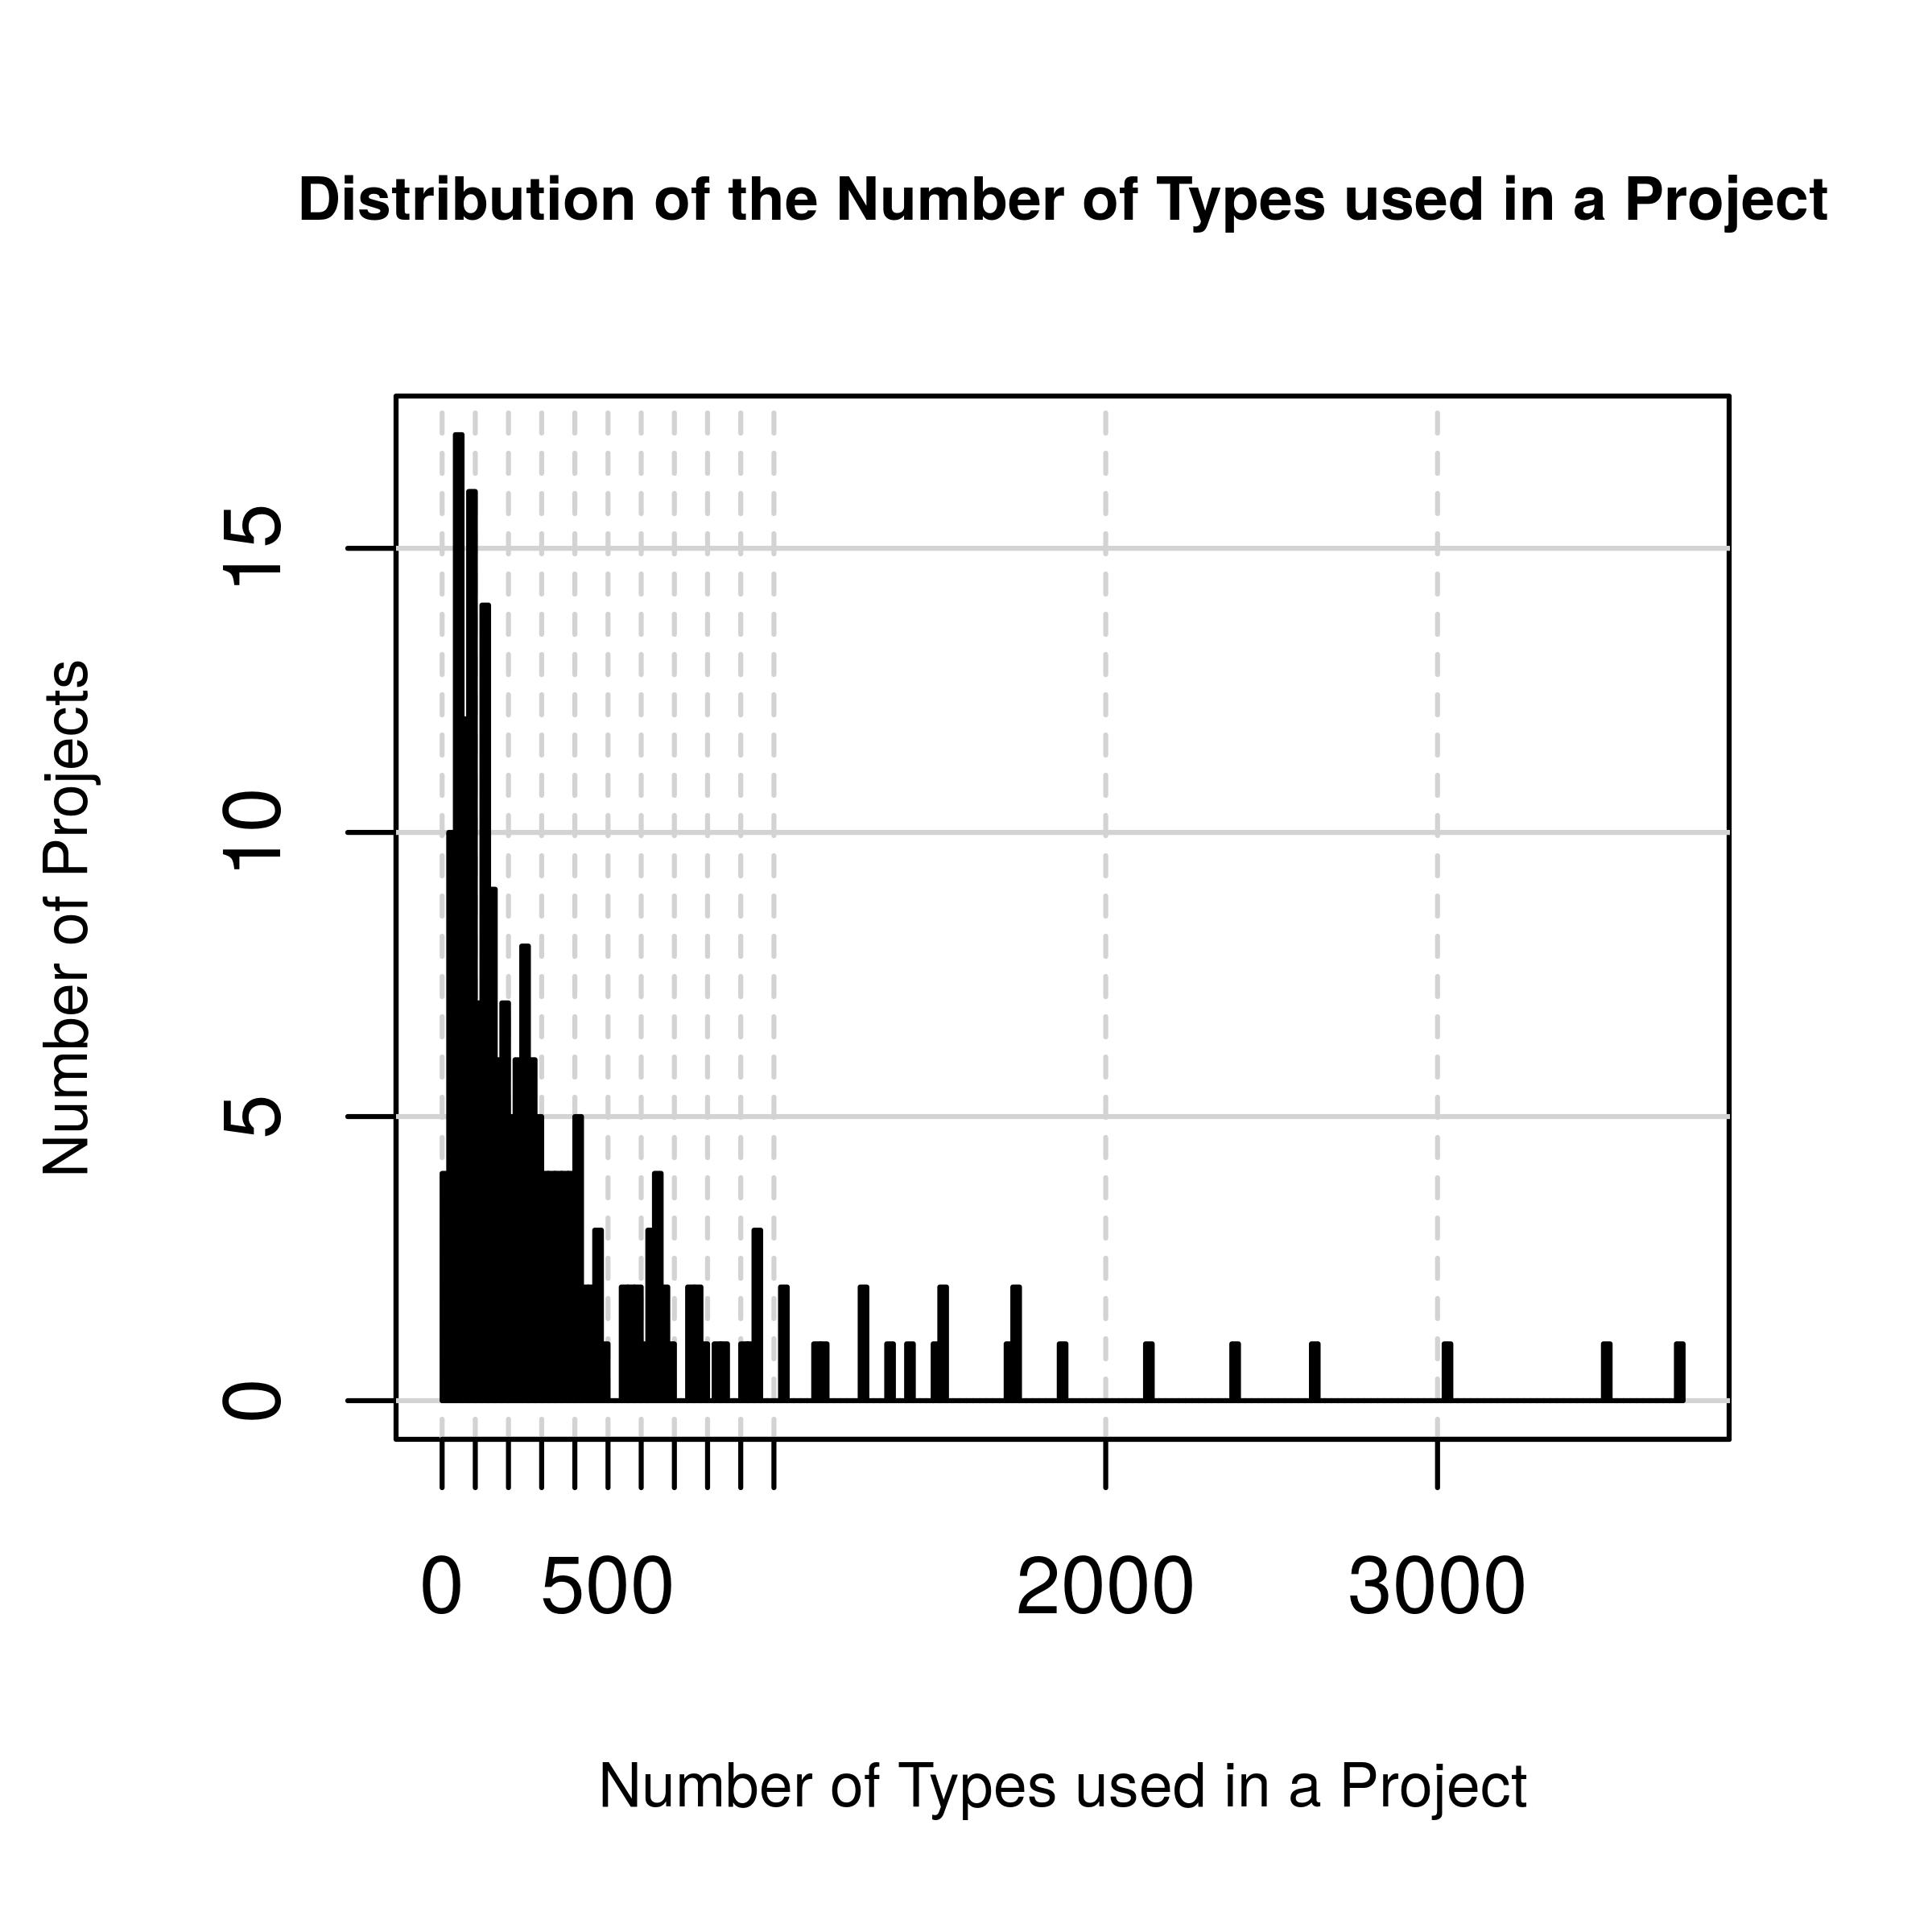
\includegraphics[height=3in, width=3in]{../lib_stats_number_of_libraries_dist}
\caption{Histogram showing the number of different types declared in a project.}
\label{lib_stats_number_of_libraries_dist}
\end{figure}

\subsection{RQ1: Do developers stick to the same types in a project?}
We found that the majority of developers declare less than 30\% of the types declared in the project. With a small group declaring more than 80\% of the types. This is shown in Figure \ref{lib_stats_dist}.

\begin{figure}[ht]
\centering
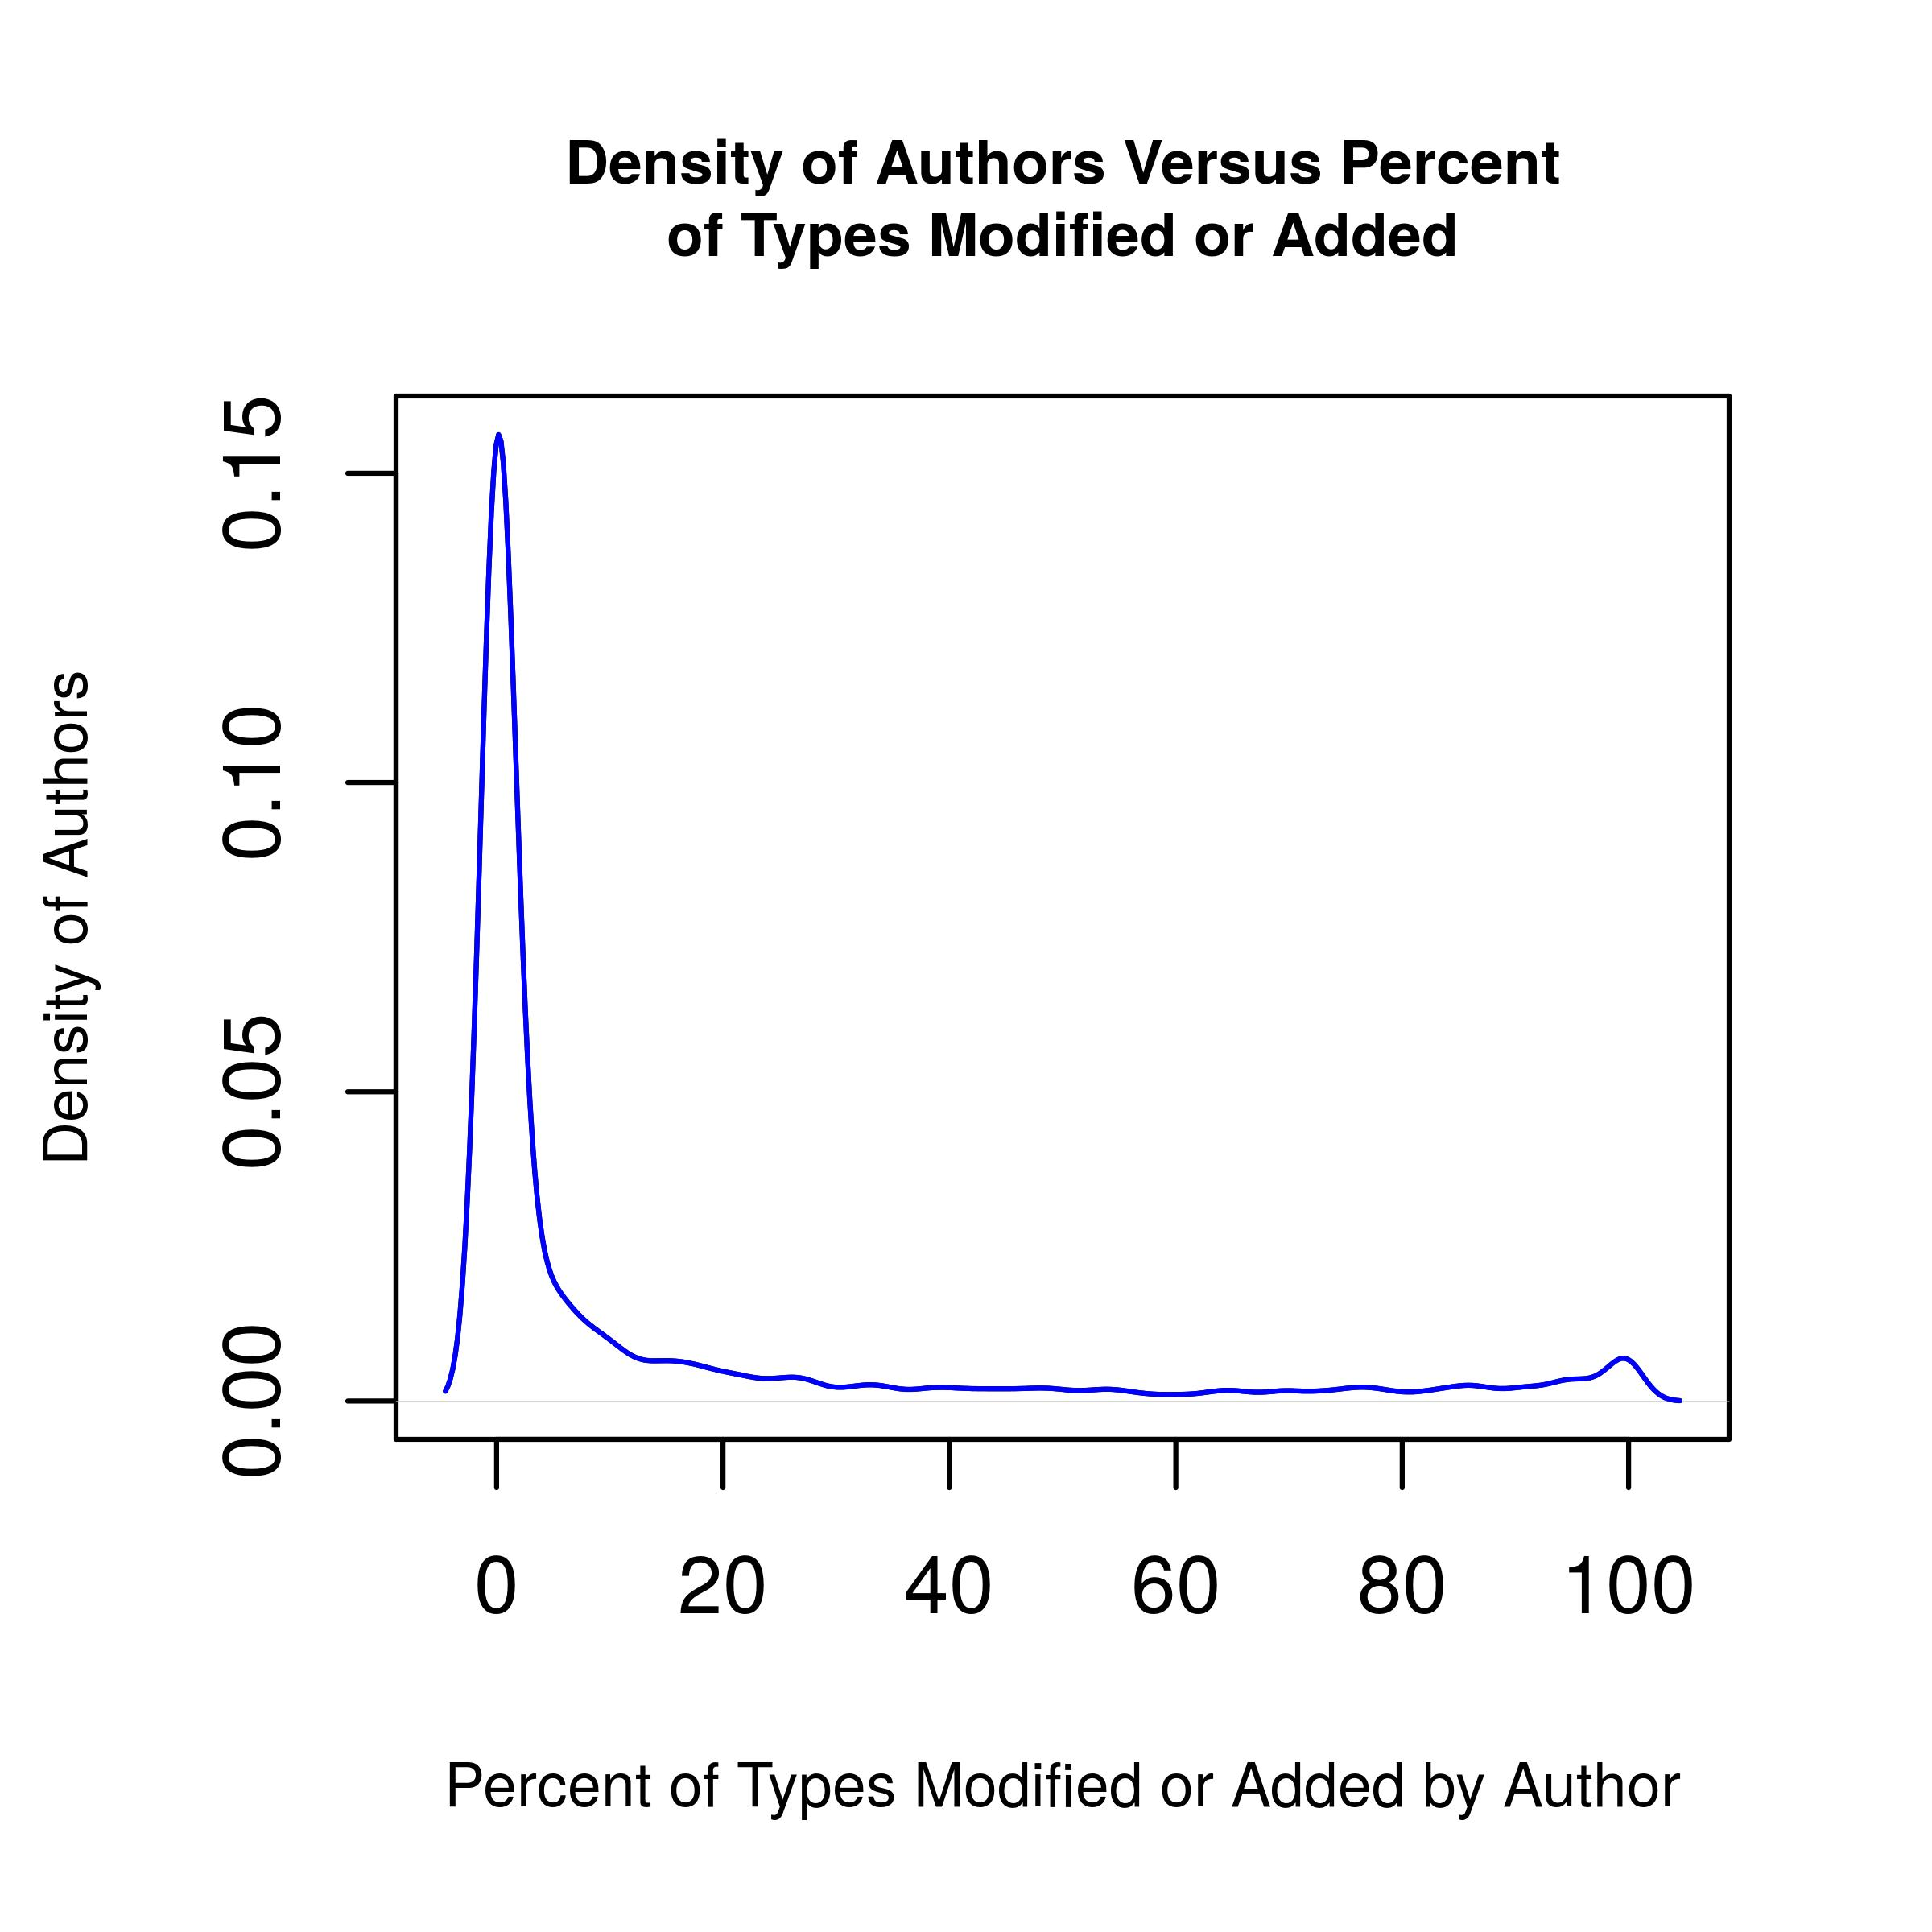
\includegraphics[height=3in, width=3in]{../lib_stats_dist}
\caption{A sample black and white graphic.}
\label{lib_stats_dist}
\end{figure}

\subsection{RQ2: How many developers in each project had large coverages?}
We found that on average a project has about 7 authors. In these projects on average only two developers modified or added over 50\% of the types used in the project. Furthermore on average only one developer modified or added over 80\% of the types. This is shown if Figures \ref{lib_stats_Threshold50_dist} and \ref{lib_stats_Threshold80_dist} respectively.

\begin{figure}[ht]
\centering
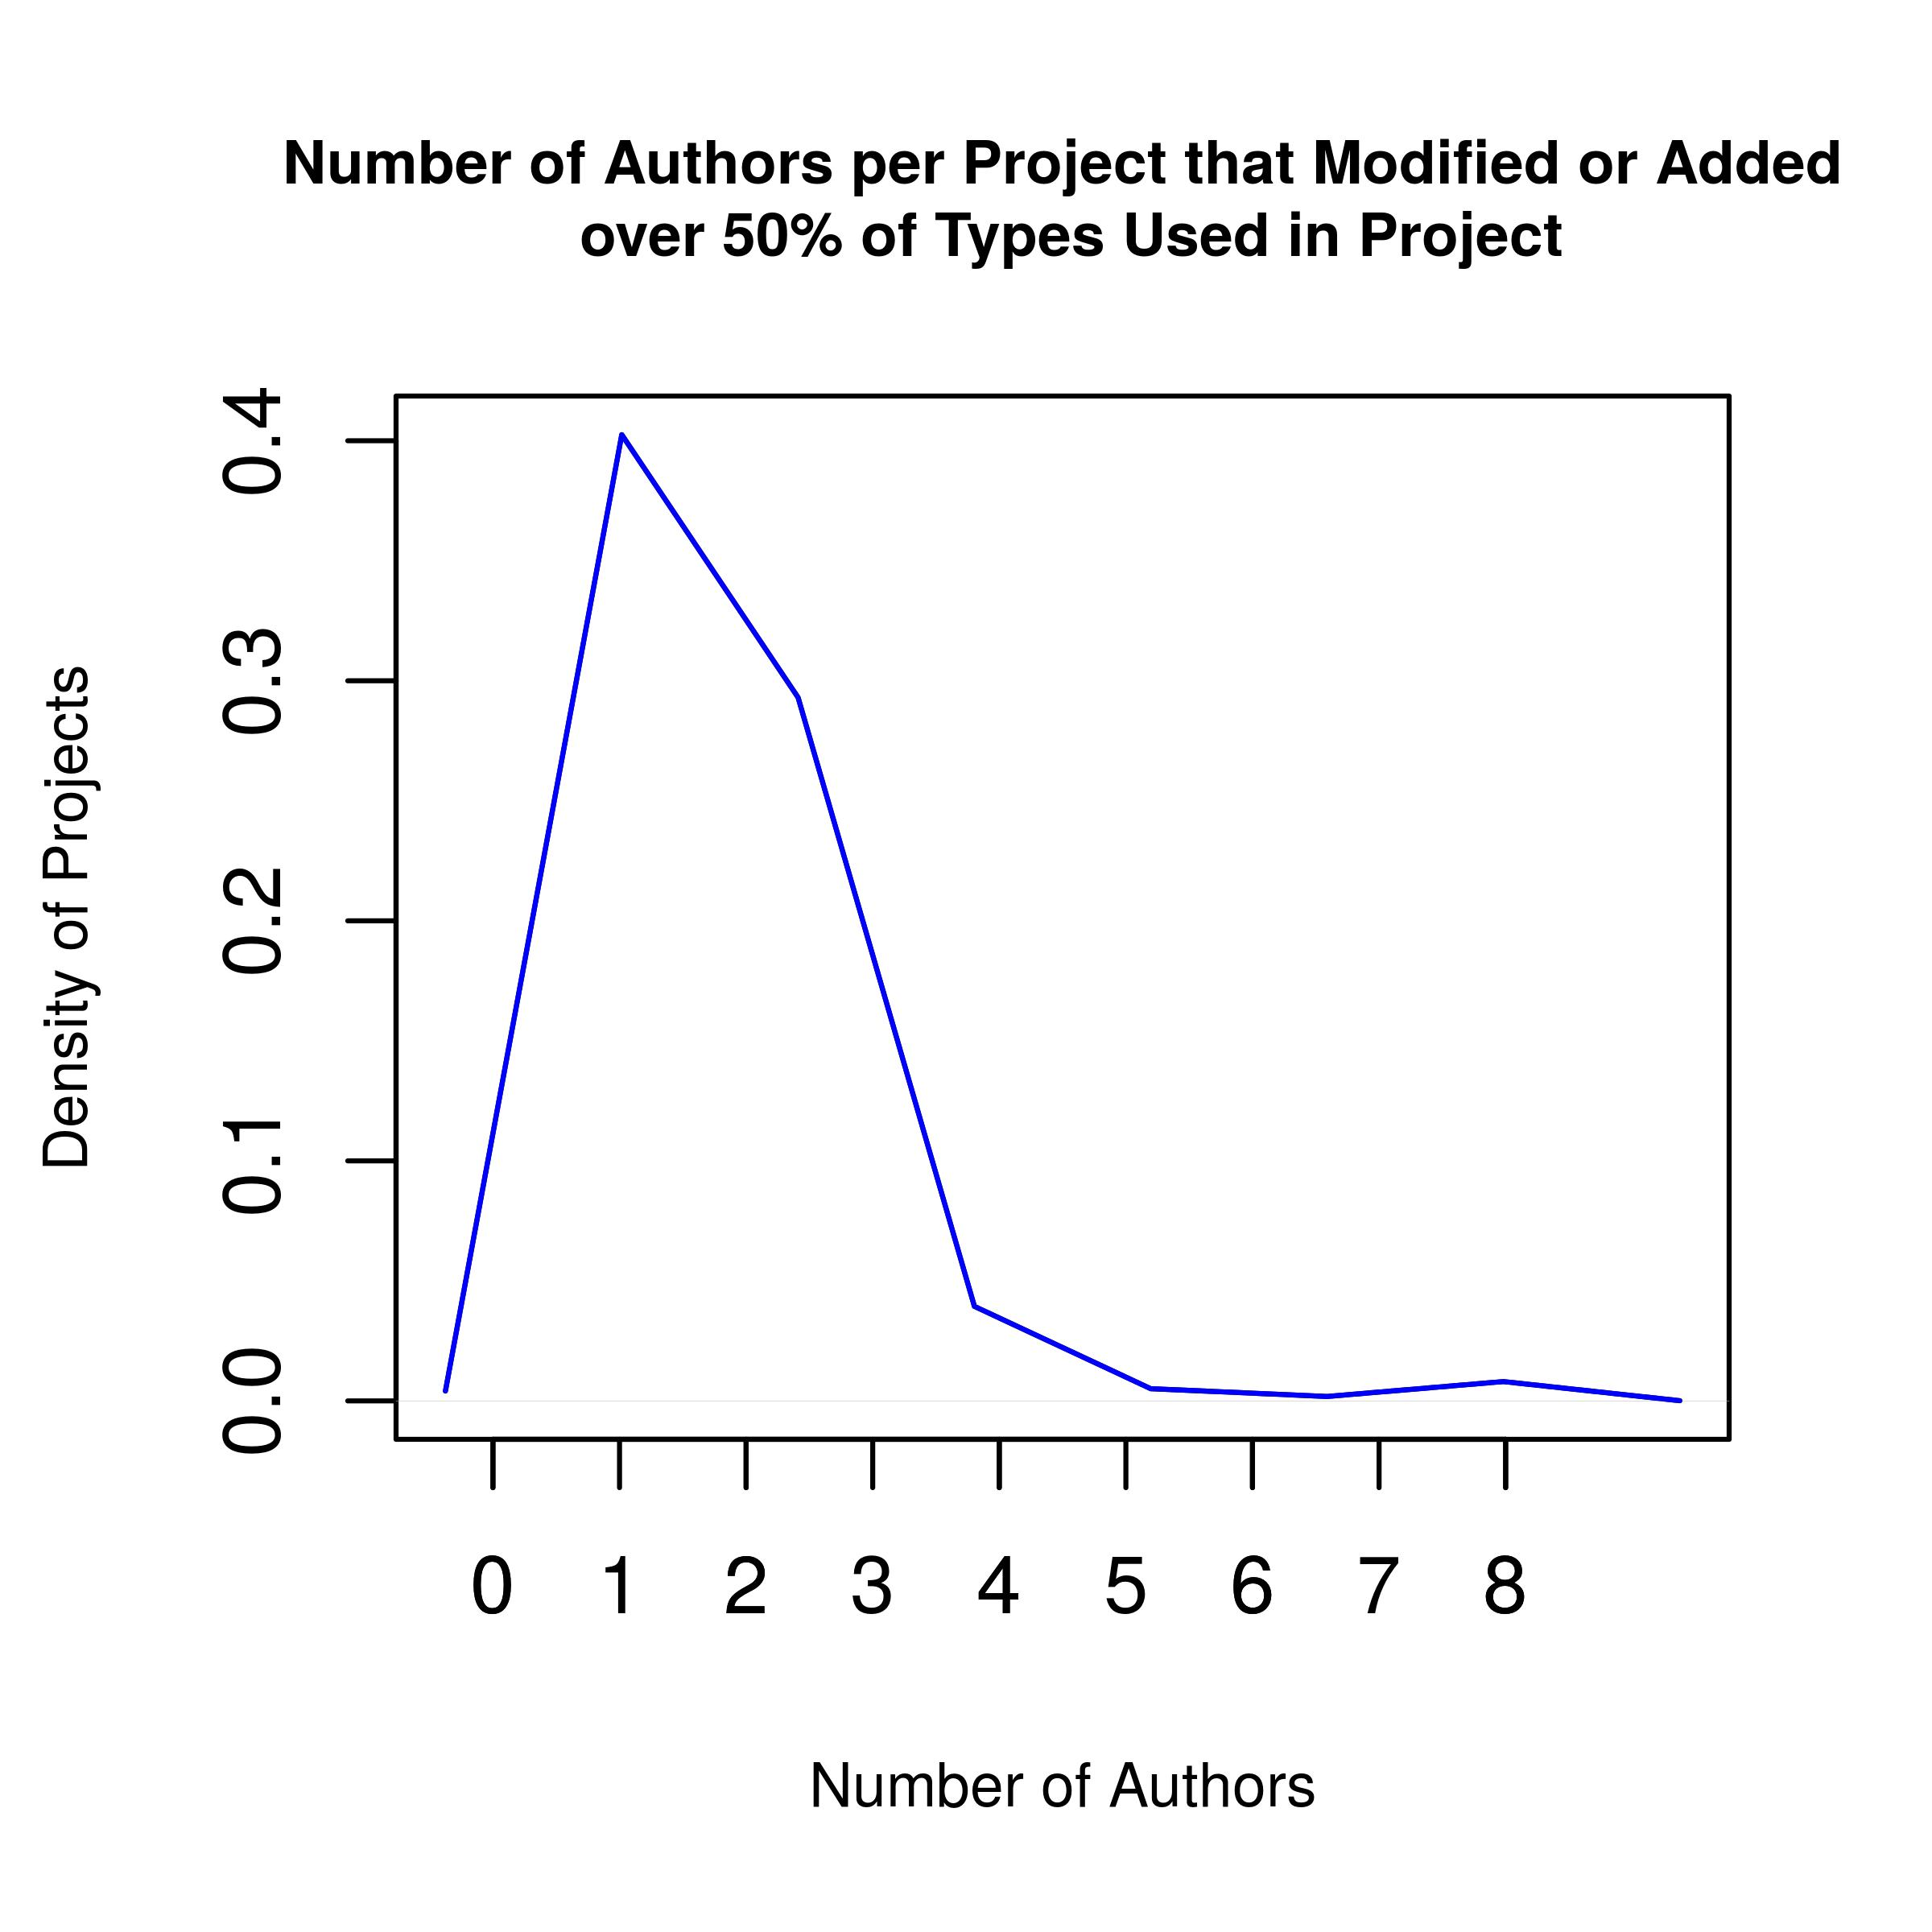
\includegraphics[height=3in, width=3in]{../lib_stats_Threshold50_dist}
\caption{A sample black and white graphic.}
\label{lib_stats_Threshold50_dist}
\end{figure}

\begin{figure}[ht]
\centering
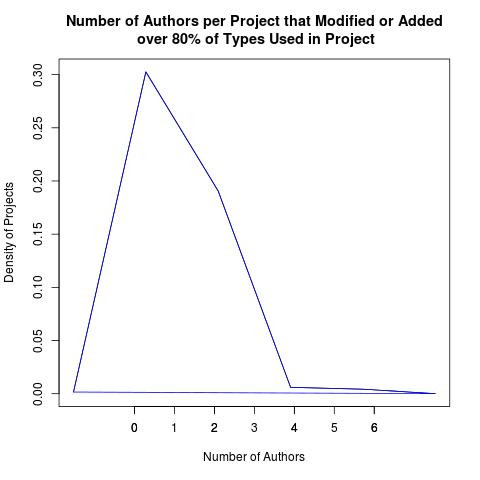
\includegraphics[height=3in, width=3in]{../lib_stats_Threshold80_dist}
\caption{A sample black and white graphic.}
\label{lib_stats_Threshold80_dist}
\end{figure}

Looking at Figure \ref{lib_stats_count_authors_percent_per_project} we can see that approximately 70\% of the projects have at least one developer who has modified or added over 90\% of the types used in a project. Furthermore all projects have at least one developer that modified or added over 50\% of the types.


\begin{figure}[ht]
\centering
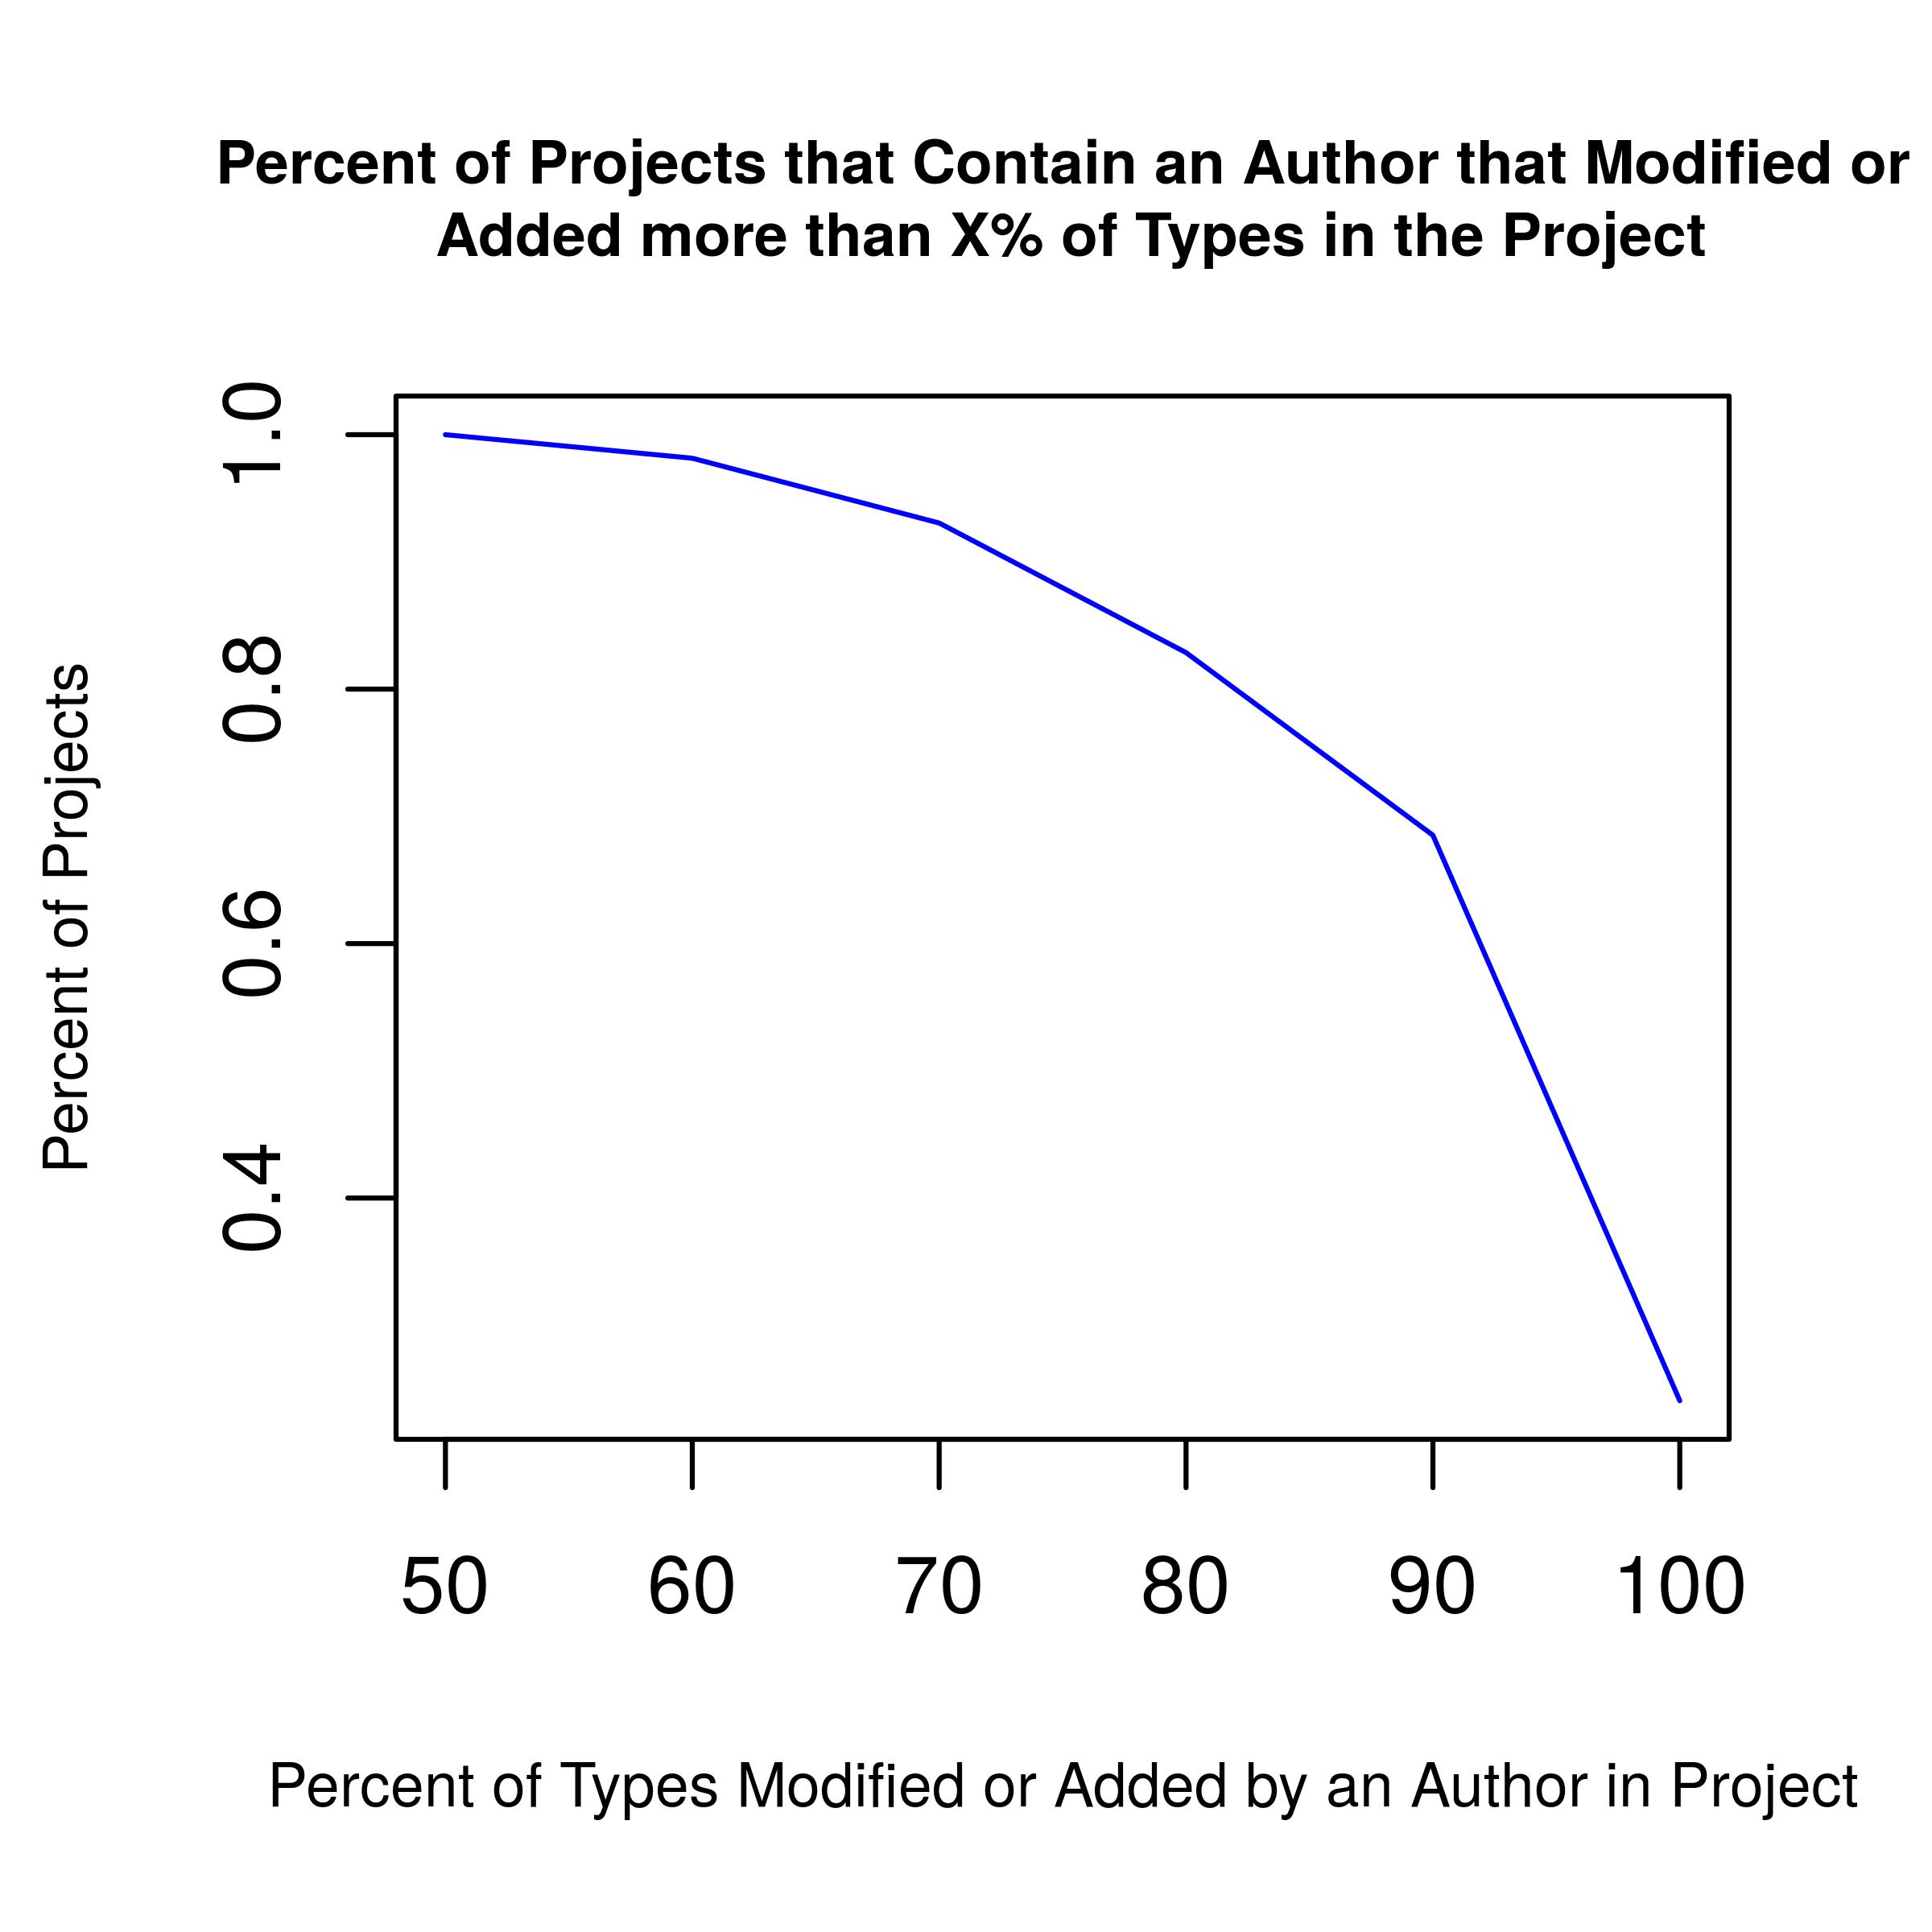
\includegraphics[height=3in, width=3in]{../lib_stats_count_authors_percent_per_project}
\caption{A sample black and white graphic.}
\label{lib_stats_count_authors_percent_per_project}
\end{figure}

\section{Conclusions and Future Work}
%\end{document}  % This is where a 'short' article might terminate

%ACKNOWLEDGMENTS are optional
\section{Acknowledgments}

%
% The following two commands are all you need in the
% initial runs of your .tex file to
% produce the bibliography for the citations in your paper.
\bibliographystyle{abbrv}
\bibliography{sigproc}  % sigproc.bib is the name of the Bibliography in this case
% You must have a proper ".bib" file
%  and remember to run:
% latex bibtex latex latex
% to resolve all references
%
% ACM needs 'a single self-contained file'!
%
%APPENDICES are optional
%\balancecolumns
\appendix
%Appendix A
\section{Headings in Appendices}

%\balancecolumns % GM June 2007
% That's all folks!
\end{document}
